% Created 2025-08-04 Mon 01:15
% Intended LaTeX compiler: lualatex
\documentclass[bigger]{beamer}
\usepackage{amsmath}
\usepackage{fontspec}
\usepackage{graphicx}
\usepackage{longtable}
\usepackage{wrapfig}
\usepackage{rotating}
\usepackage[normalem]{ulem}
\usepackage{capt-of}
\usepackage{hyperref}
\usetheme[progressbar=foot, sectionpage=none, numbering=fraction]{metropolis}
\usepackage{tikz}
\usepackage{booktabs}
\usepackage{adjustbox}
\usepackage{diagbox}
\usepackage{latexcolors}
\usetikzlibrary{automata, positioning, arrows, arrows.meta}
\usepackage{diagbox}
\usepackage{dsfont}
\usepackage{amsmath}
\usepackage{fontawesome}
\usepackage{pgfgantt}
\usepackage[ruled]{algorithm2e}
\usepackage[absolute, overlay]{textpos}
\usepackage{xcolor}
\definecolor{UmlBlue}{HTML}{0067b1} \setbeamercolor{progress bar}{fg=UmlBlue} \setbeamercolor{title separator}{fg=UmlBlue}
\setbeamercolor{progress bar in head/foot}{fg=UmlBlue} \setbeamercolor{progress bar in section page}{fg=UmlBlue} \setbeamercolor{alerted text}{fg=UmlBlue}
\definecolor{RedBrown}{RGB}{192, 4, 4}
\pretocmd{\tableofcontents}{\thispagestyle{empty}}{}{}
\usepackage{listings}
\usepackage{multimedia}
\usepackage[all]{foreign}
\usetheme{default}
\author{Andrea Pierré}
\date{August 04, 2025}
\title{\emph{Robust representations for olfactory-spatial association learning}}
\setbeamercovered{transparent=10}
\setbeamertemplate{section in toc}[sections numbered]
\AtBeginSection[]{\begin{frame}[plain, noframenumbering]{Outline}    \setbeamertemplate{section in toc}[sections numbered]\setbeamertemplate{subsection in toc}[subsections numbered]\tableofcontents[currentsection, currentsubsection]\end{frame}}
\AtBeginSubsection[]{\begin{frame}[plain, noframenumbering]{Outline}\setbeamertemplate{section in toc}[sections numbered]\setbeamertemplate{subsection in toc}[subsections numbered]\tableofcontents[currentsection,currentsubsection]\end{frame}}
\definecolor{headercolor}{HTML}{232323}
\setbeamercolor{normal text}{%
% bg=,
fg=headercolor
}
\hypersetup{
 pdfauthor={Andrea Pierré},
 pdftitle={\emph{Robust representations for olfactory-spatial association learning}},
 pdfkeywords={},
 pdfsubject={},
 pdfcreator={Emacs 30.1 (Org mode 9.7.31)}, 
 pdflang={English}}
\begin{document}

\maketitle
\begin{frame}[plain]{Outline}
\tableofcontents
\end{frame}

\section{Project recap}
\label{sec:orgae57615}
\begin{frame}[label={sec:org11e8010}]{The LEC is key to sensory associations and spatial memory}
\begin{columns}
\begin{column}{0.45\columnwidth}
\footnotesize
\begin{itemize}
\item \alert{Piriform Cortex} encodes olfactory information
\item \alert{Hippocampus} encodes spatial information
\item \alert{Lateral Entorhinal Cortex (LEC)} encodes both olfactory \& spatial information
\end{itemize}
\end{column}
\begin{column}{0.55\columnwidth}
\begin{center}
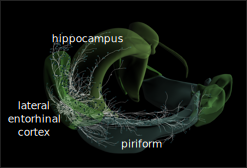
\includegraphics[width=\textwidth]{medias/brain.png}
\end{center}

\begin{textblock}{5}(0.5,14.5)%
\tiny
Poo et al., 2022\\
Bitzenhofer et al., 2022\\
Lee et al., 2021
\end{textblock}
\end{column}
\end{columns}
\end{frame}
\begin{frame}[label={sec:org72bed81}]{Half triangle task for olfactory-spatial association learning}
\begin{columns}
\begin{column}[c]{0.33\columnwidth}
\begin{center}
\movie{\includegraphics[width=\linewidth, keepaspectratio, trim={0cm 0cm 28cm 0cm}, clip]{medias/video-picture.png}}{medias/annotatedF03_d35_2022-11-15_15.41.mp4}
\end{center}
\end{column}
\begin{column}[c]{0.33\columnwidth}
\begin{center}
East/West task
\includegraphics[width=0.9\linewidth, keepaspectratio, trim={11cm 18cm 40cm 13cm}, clip]{medias/task-east-west.png}
\end{center}
\end{column}
\begin{column}[c]{0.33\columnwidth}
\begin{center}
Left/Right task
\includegraphics[width=0.9\linewidth, keepaspectratio, trim={3cm 2cm 4cm 4cm}, clip]{medias/task-left-right.jpeg}
\end{center}
\end{column}
\end{columns}
\end{frame}
\begin{frame}[label={sec:orgcb37737}]{Deep Reinforcement Learning model}
\begin{columns}
\begin{column}[c]{0.5\columnwidth}
\begin{center}
\includegraphics[height=0.9\textheight]{medias/nn.drawio.png}
\end{center}
\end{column}
\begin{column}[c]{0.5\columnwidth}
\pause
\begin{itemize}
\item Agent learns a policy (sequences of actions) that maximize rewards
\end{itemize}
\pause
\begin{itemize}
\item RL \(\to\) no need to have ground truth data (as in supervised learning)
\end{itemize}
\end{column}
\end{columns}
\end{frame}
\begin{frame}[label={sec:orgdb679ef}]{The environment}
\begin{center}
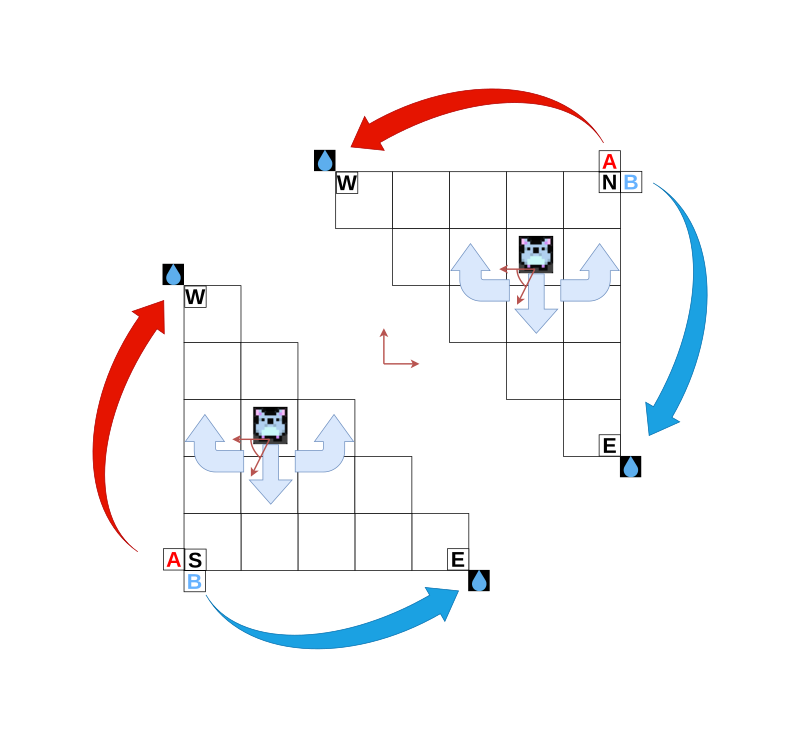
\includegraphics[height=0.6\textheight]{medias/RL_env-cartesian-polar.drawio.png}
\end{center}
\footnotesize
\vspace{-1em}
\begin{itemize}
\item 3 actions: \(\Leftarrow \quad \Uparrow \quad \Rightarrow\)
\item \alert{Duplicated} coordinates inputs:
\begin{itemize}
\item Cartesian coordinates from north \& south port
\item Polar coordinates from north \& south port
\end{itemize}
\end{itemize}
\end{frame}
\begin{frame}[label={sec:orga34c87a}]{Questions \& Hypothesis}
\metroset{block=fill}
\begin{exampleblock}{Questions}
\begin{itemize}
\footnotesize
\setlength\itemsep{0em}
\item What \alert{function} does the network learn?
\item How the constrains of the task affect learning \& the representations learned?
%\item How this task structure might employ different representations of the action space?
\item How do the representations learned compare between the \emph{in vivo} and the \emph{in silico} neurons?
\end{itemize}
\end{exampleblock}
\pause
\begin{exampleblock}{Hypothesis}
\begin{itemize}
\footnotesize
\setlength\itemsep{0em}
\item The network will use the \alert{most efficient coordinate information} (Cartesian vs. polar) based on the task (left/right vs. east/west)
\item The structure of the network's weights will reflect this prioritization of information
\item Some neurons will encode a \alert{joint representation of \{odor \& space\}} (\ie{} conjunctive cells)
\end{itemize}
\end{exampleblock}
\end{frame}
\section{Modeling \& Simulation}
\label{sec:orgbc9a86c}
\begin{frame}[label={sec:org89a78da}]{State space \& network architecture}
\begin{center}
\includegraphics[height=0.95\textheight]{medias/NN-architecture-MLP.drawio.png}
\end{center}
\end{frame}
\begin{frame}[label={sec:orgc9c9fa1}]{Training}
East/West
\begin{center}
\includegraphics[height=0.35\textheight]{medias/EastWest/training.png}
\end{center}
Left/Right
\begin{center}
\includegraphics[height=0.35\textheight]{medias/LeftRight/training.png}
\end{center}
\end{frame}
\begin{frame}[label={sec:orgffc63ac}]{Agent behavior}
\begin{columns}
\begin{column}[t]{0.33\columnwidth}
\begin{center}
\small
Naive agent\\[1em]
\movie{\includegraphics[width=\linewidth, keepaspectratio]{medias/simulations/LeftRight100to150.jpg}}{medias/simulations/LeftRight100to150.mp4}
\end{center}
\end{column}
\begin{column}[t]{0.33\columnwidth}
\begin{center}
\small
Intermediate agent\\[1em]
\movie{\includegraphics[width=\linewidth, keepaspectratio]{medias/simulations/LeftRight200to250.jpg}}{medias/simulations/LeftRight200to250.mp4}
\end{center}
\end{column}
\begin{column}[t]{0.33\columnwidth}
\begin{center}
\small
Trained agent\\[1em]
\movie{\includegraphics[width=\linewidth, keepaspectratio]{medias/simulations/LeftRight300to350.jpg}}{medias/simulations/LeftRight300to350.mp4}
\end{center}
\end{column}
\end{columns}
\end{frame}
\section{Results}
\label{sec:org9a2b5c4}
\begin{frame}[label={sec:org8bb0ba1}]{Pre-odor activations cluster together -- East/West}
\begin{center}
\includegraphics[height=0.9\textheight]{medias/activations-learned-EastWest.png}
\end{center}
\end{frame}
\begin{frame}[label={sec:org95631fe}]{Pre-odor activations cluster together -- Left/Right}
\begin{center}
\includegraphics[height=0.9\textheight]{medias/activations-learned-LeftRight.png}
\end{center}
\end{frame}
\begin{frame}[label={sec:org9a95a04}]{PCA on activations by layer on \(\{x, y\}\) coordinates -- Left/Right}
\begin{textblock}{15}(0.5, 3.5)%
\includegraphics[height=0.7\textheight, keepaspectratio]{medias/PCA-layers-activations-coords-LeftRight.png}
\vspace{-2em}
\footnotesize
\begin{itemize}
\setlength\itemsep{0em}
\item From grid shape in early layer to half moon cluster in late layers
\item Seems to encode the lower/upper triangle
\end{itemize}
\end{textblock}
\end{frame}
\begin{frame}[label={sec:orgada7815}]{PCA on activations by layer on odor cue -- Left/Right}
\begin{textblock}{15}(0.2, 3.5)%
\includegraphics[height=0.68\textheight, keepaspectratio]{medias/PCA-layers-activations-cue-LeftRight.png}
\vspace{-2em}
\footnotesize
\begin{itemize}
\setlength\itemsep{0em}
\item From grid shape in early layer to half moon cluster in late layers
\item Seems that odor cues cluster by tile/grid
\end{itemize}
\end{textblock}
\end{frame}
\begin{frame}[label={sec:org522d681}]{Cartesian inputs unchanged -- polar inputs perturbed}
\begin{columns}
\begin{column}[c]{0.5\columnwidth}
\begin{center}
\small
\textbf{East/West}\\
\footnotesize
Silencing inputs
\end{center}
\begin{center}
\includegraphics[width=\textwidth]{medias/EastWest/exp_keep-cartesian_silence-True.png}
\end{center}
\begin{center}
\footnotesize
Randomizing inputs
\end{center}
\begin{center}
\includegraphics[width=\textwidth]{medias/EastWest/exp_keep-cartesian_silence-False.png}
\end{center}
\end{column}
\begin{column}[c]{0.5\columnwidth}
\begin{center}
\small
\textbf{Left/Right}\\
\footnotesize
Silencing inputs
\end{center}
\begin{center}
\includegraphics[width=\textwidth]{medias/LeftRight/exp_keep-cartesian_silence-True.png}
\end{center}
\begin{center}
\footnotesize
Randomizing inputs
\end{center}
\begin{center}
\includegraphics[width=\textwidth]{medias/LeftRight/exp_keep-cartesian_silence-False.png}
\end{center}
\end{column}
\end{columns}
\end{frame}
\begin{frame}[label={sec:org4507a69}]{Polar inputs unchanged -- Cartesian inputs perturbed}
\begin{columns}
\begin{column}[c]{0.5\columnwidth}
\begin{center}
\small
\textbf{East/West}\\
\footnotesize
Silencing inputs
\end{center}
\begin{center}
\includegraphics[width=\textwidth]{medias/EastWest/exp_keep-polar_silence-True.png}
\end{center}
\begin{center}
\footnotesize
Randomizing inputs
\end{center}
\begin{center}
\includegraphics[width=\textwidth]{medias/EastWest/exp_keep-polar_silence-False.png}
\end{center}
\end{column}
\begin{column}[c]{0.5\columnwidth}
\begin{center}
\small
\textbf{Left/Right}\\
\footnotesize
Silencing inputs
\end{center}
\begin{center}
\includegraphics[width=\textwidth]{medias/LeftRight/exp_keep-polar_silence-True.png}
\end{center}
\begin{center}
\footnotesize
Randomizing inputs
\end{center}
\begin{center}
\includegraphics[width=\textwidth]{medias/LeftRight/exp_keep-polar_silence-False.png}
\end{center}
\end{column}
\end{columns}
\end{frame}
\begin{frame}[label={sec:org8212a43}]{Bottleneck network \(\to\) performance degrades below \(\sim\!10\) neurons}
\begin{center}
\includegraphics[height=0.4\textheight]{medias/NN-architecture-bottleneck.drawio.png}
\end{center}
\vspace{-3em}
\begin{columns}
\begin{column}[c]{0.5\columnwidth}
\begin{center}
\small
\textbf{East/West}\\
\end{center}
\begin{center}
\includegraphics[width=0.9\textwidth]{medias/steps-boxplot-EastWest.png}
\end{center}
\end{column}
\begin{column}[c]{0.5\columnwidth}
\begin{center}
\small
\textbf{Left/Right}\\
\end{center}
\begin{center}
\includegraphics[width=0.9\textwidth]{medias/steps-boxplot-LeftRight.png}
\end{center}
\end{column}
\end{columns}
\end{frame}
\section{Conclusion}
\label{sec:org66bca22}
\begin{frame}[<+->][label={sec:org55e3f32}]{Partial conclusions so far}
\begin{itemize}
\item The \alert{pre-odor activations} cluster together, but no other clear pattern seems to emerge
\item Dimensionality reduction analysis \(\to\) the network seems to mainly encode the \alert{position of the agent on the grid}
\item With this task setup, it seems \alert{both types of coordinates information are required} to solve the task \(\to\) is this a negative result that invalidates our original hypothesis or is this due to overfitting?
\begin{itemize}
\item From earlier experiments, we know the agent can perfectly solve the task without needing duplicated inputs\(\text{\dots}\)
\end{itemize}
\end{itemize}
\end{frame}
\begin{frame}[<+->][label={sec:org964d3f9}]{Next steps}
\begin{itemize}
\item What happens in between tiles? Did the network learn to interpolate?
\item Add dropout during training to make the network more robust to perturbations and avoid overfitting?
\item Identify the potential functions of the neurons in the bottleneck layer? What type of information do they encode? Any sign of potential conjunctive cells?
\item End of this project \(\to\) still looking for well defined results/principes/rules for a potential MVP (Minimum Viable Publication)
\end{itemize}
\end{frame}
\begin{frame}[label={sec:orgd42eafa},standout]{~}
Questions ?
\end{frame}
\appendix
\begin{frame}[fragile]{Pytorch network}
\addtocounter{framenumber}{-1}
\scriptsize
\begin{lstlisting}
DQN(
  (mlp): Sequential(
    (0): Linear(in_features=21, out_features=512, bias=True)
    (1): Linear(in_features=512, out_features=512, bias=True)
    (2): ReLU()
    (3): Linear(in_features=512, out_features=512, bias=True)
    (4): ReLU()
    (5): Linear(in_features=512, out_features=512, bias=True)
    (6): ReLU()
    (7): Linear(in_features=512, out_features=3, bias=True)
  )
)
\end{lstlisting}
\end{frame}
\end{document}
